\subsection{Glyphs: \glyph{Clone markers}}
\label{sec:cloneMarker}

If an \glyph{EPN} is duplicated on a map, it is necessary to indicate this fact by using the \glyph{clone marker} auxiliary unit.
The purpose of this marker is to provide the reader with a visual indication that this node has been cloned, and that at least one other occurrence of the \glyph{EPN} can be found in the map (or in a submap; see \sect{submap}).
The clone marker takes two forms, simple and labelled, depending on whether the node being cloned can carry state variables (\ie whether it is a stateful EPN).
Note that an \glyph{EPN} belongs to a single compartment.
If two glyphs labelled ``X'' are located in two different compartments, such as an EPN labelled ``ATP'' in the cytosol, and another EPN labelled ``ATP'' in the mitochondrial lumen, they represent different \glyph{EPNs} and therefore do not need to be marked as cloned.

\subsubsection{\glyph{Simple clone marker}}

\begin{glyphDescription}

\glyphSboTerm
Not applicable.

\glyphIncoming
None.

\glyphOutgoing
None.

\glyphContainer
A \glyph{simple clone marker} is represented by a portion of the surface of an \glyph{EPN} that has been modified visually through the use of a different shade, texture, or colour, as shown in \fig{simpleCloneMarker}.
The \glyph{simple clone marker} occupies the lower part of the \glyph{EPN}.
The filled area must be smaller than the unfilled one.

\glyphLabel
None.

\glyphAux
None.

\end{glyphDescription}

\begin{figure}[H]
  \centering
  
\includegraphics{images/build/simple_clone_marker.pdf}
  \caption{The \PD glyph for \glyph{simple clone marker} applied to a \glyph{simple chemical} and a \glyph{multimer} of \glyph{simple chemicals}.}
  \label{fig:simpleCloneMarker}
\end{figure}

\fig{example-cloning} contains an example in which we illustrate the use of \glyph{simple clone markers} to clone ATP and ADP participating in different processes.  This example also demonstrates the chief drawbacks of using clones: it leads to a kind of dissociation of the overall network and multiplies the number of nodes required, requiring more work on the part of the reader to interpret the result.  Sometimes these disadvantages are offset in larger maps by a reduction in the overall number of line crossings, but not always.  In general, we advise that cloning should be used sparingly.

\begin{figure}[H]
  \centering
  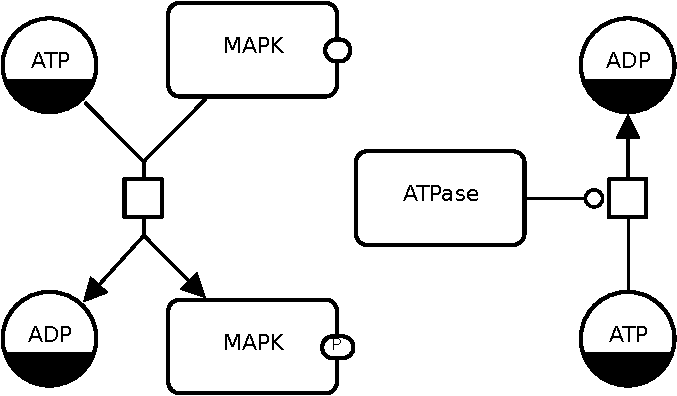
\includegraphics[scale = 0.8]{images/build/cloning_example.pdf}
  \caption{An example of using cloning, here for ATP and ADP.}
  \label{fig:example-cloning}
\end{figure}

\subsubsection{\glyph{Labelled clone marker}}

Unlike the \glyph{simple clone marker}, the \glyph{labelled clone marker} includes (unsurprisingly, given its name) an identifying label that can be used to identify equivalent clones elsewhere in the map.
This is particularly useful for stateful \glyph{EPNs} because these can have a large number of state variables displayed and therefore may be difficult to identify as being identical visually.
All duplicated stateful EPNs must be decorated with a \glyph{labelled clone marker}.

\begin{glyphDescription}

\glyphSboTerm Not applicable.

\glyphIncoming
None.

\glyphOutgoing
None.

\glyphContainer
The \glyph{labelled clone marker} is represented by a portion of the surface of an \glyph{EPN} that has been modified visually through the use of a different shade, texture, or colour, as shown in \fig{labelledCloneMarker}.
The \glyph{labelled clone marker} occupies the lower part of the \glyph{EPN}.
The filled area must be smaller than the unfilled one, but be large enough to accommodate the \glyph{labelled clone marker}'s label.

\glyphLabel
A \glyph{labelled clone marker} is identified by a label that is  a string of characters that may be distributed on several lines to improve readability.
The centre of the label must be placed on the centre of the container.
The label may extend outside of the container.
The font colour of the label and the colour of the \glyph{labelled clone marker} should contrast with one another.
The label on a \glyph{labelled clone marker} is mandatory.

\glyphAux
None.

\end{glyphDescription}

\begin{figure}[H]
  \centering
  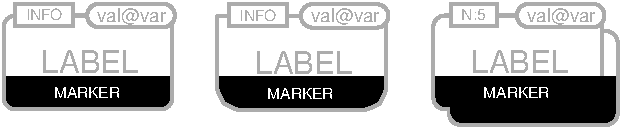
\includegraphics{images/build/labeled_clone_marker.pdf}
  \caption{The \PD glyph for \glyph{labelled clone marker} applied to a \glyph{macromolecule}, a \glyph{nucleic acid feature} and a \glyph{multimer} of \glyph{macromolecules}.}
  \label{fig:labelledCloneMarker}
\end{figure}
